% Intro
This chapter, divided into three sections, provides an overview of the project’s context. The first section introduces Oracle Corporation, the host organisation, providing insights into its history, field of activity, services, organizational structure, and culture. The second section explores the framework of the project, outlining the team in which it took place, the topic overview, to problematic it solves and the objectives to be achieved. The final section focuses on project management, including agile practices and collaboration tools, and the internship planning process.
\newpage
\fancyhead[R]{\textsc{Chapter 1 - General Context of the project}}

% Host Organization
\section{Host Organization}

My internship was hosted by Oracle Corporation, specifically Oracle Morocco Research \& Development Center. This section introduces both entities, providing insights into their history and services.

% Presentation
\subsection{Presentation}
In today's world, businesses, technology companies, and the public sector rely on databases to store their data, while utilizing cloud services to manage their IT infrastructure and other essential tools such as ERP (Enterprise Resource Planning), CRM (Customer Relationship Management), EPM (Enterprise Performance Management), and SCM (Supply Chain Management). These technologies have taken a crucial role, making it inconceivable to function without them.\mynewline

Oracle, a leading US multinational computer technology corporation, not only employs these tools in its day-to-day operations but also creates and provides them to customers. Moreover, the company places a high value on innovation and ensuring customer satisfaction.\mynewline

The first part of this section provides a broad context by giving an overview of Oracle Corporation and Oracle Morocco Application \& Development Center (MADC). This includes an understanding of their business area of activity, their mission, as well as their organizational culture, and structure.

% Oracle Corporation
\subsection{Oracle Corporation}
\begin{center}
    \centering
    
\includegraphics[width=0.5\textwidth]{Images/oracle_corp_logo.jpg}
    \captionof{figure}{Oracle Logo} \cite{O-History}
    \label{fig:oracle}
\end{center}

% History
\subsubsection{History}
Oracle Corporation is a Tech company with headquarters in Austin, Texas. In 1977, Larry Ellison, Bob Miner, and Ed Oates founded Oracle Corporation, then called as Software Development Laboratories (SDL). The company first focused on creating Oracle Database, a relational database management system (RDBMS), that became its flagship product. Enterprise software, cloud computing, hardware systems, and consulting services are now all part of Oracle's growing list of services and product options. Sun Microsystems was a key acquisition in 2010, giving Oracle access to technologies such as Java and the Solaris operating system.\cite{O-History}\mynewline

Today, Oracle is a leading provider of cloud-based IT infrastructure and software that helps organizations grow, find new sources of efficiency, and improve their performance. To help organize and secure client data, Oracle developed the first and only autonomous database in the world as well as Oracle cloud.

% Business area of activity
\subsubsection{Business area of activity}
Oracle provides a variety of goods and services to its clients. Software development tools, cloud services, training, consultancy, and credentials are just a few of the goods and services offered here. One of the brands Oracle offers is Oracle Database, which has held the top spot since 1979 and is supported by cloud artificial intelligence. SaaS (Software as a Service), PaaS (Platform as a Service), IaaS (Infrastructure as a Service), and DaaS (Data as a Service) are just a few of the integrated solutions offered by Oracle Cloud Infrastructure for business, IT, and development needs.\mynewline

Oracle Middleware is also a platform that is integrated for creating and running intelligent, agile applications while increasing technical efficiency using contemporary software designs. Oracle Services, which include Oracle Advanced Customer Support Services, Oracle Premium Support, Oracle Consulting, Oracle Financing, and Oracle Managed Cloud Services.

% Oracle Labs
\subsubsection{Oracle Labs}
The research and development division of Oracle is called Oracle Labs, which focuses primarily on creating technologies that will keep Oracle at the forefront of the IT industry. Researchers at Oracle Labs pursue innovative methodologies and approaches, frequently taking on challenges or projects that would be difficult to complete within a product development organization or that involved high risk or uncertainty. \mynewline
\begin{center}
    \centering
    
\includegraphics[width=0.3\textwidth]{Images/oracle_labs_logo.jpg}
    \captionof{figure}{Oracle Labs Logo} \cite{oracle-labs}
    \label{fig:labs}
\end{center}

Real-world applications are the focus of Oracle Labs research, and the researchers are working to create technologies that will eventually have a big impact on how society and technology evolve. For instance, work done in Oracle Labs led to the development of chip multithreading and the Java computer language.\mynewline

Oracle's quest for research and development is greatly supported by Oracle Labs. Oracle can recognize challenges, find creative solutions, and create new products that can spur growth and innovation in the future because of its well-rounded research portfolio.

% Oracle MADC
\subsubsection{Oracle MADC}
The first Oracle R\&D center in Africa and one of only a few in the world, the Oracle MADC Morocco Research and Development Center, is a software development center established by Oracle Corporation in Casablanca, Morocco.\mynewline
\begin{center}
    \centering
    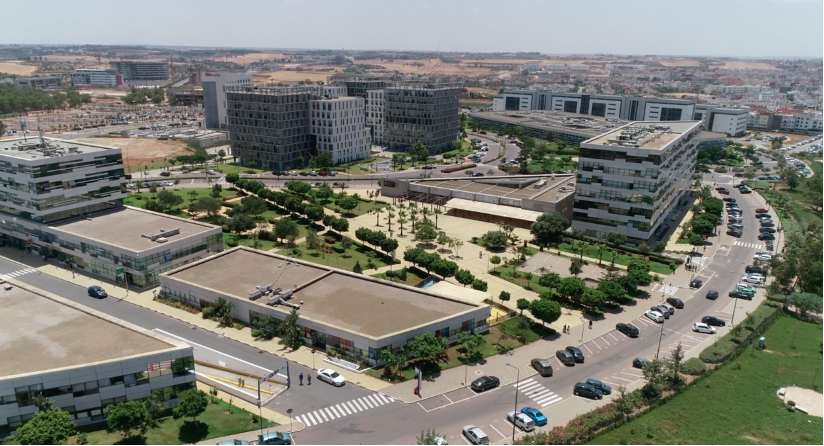
\includegraphics[width=\textwidth]{Images/nearshore oracle.png}
    \captionof{figure}{Oracle MADC Location}
    \label{fig:casa}
\end{center}
\noindent
\mynewline
The center was inaugurated in 2015 and is one of Oracle's key development centers in the EMEA region (Europe, Middle East, and Africa). The center is staffed by highly skilled and talented software developers, engineers, and project managers who work on a variety of projects across various Oracle product lines utilizing the newest trends in innovation, such as artificial intelligence, augmented/virtual/mixed reality, big data analytics, Blockchain, cloud computing, cybersecurity, internet of things, machine learning, mobile computing, serverless computing. The center's researchers make use of all these technologies to tackle the most pressing problems facing business, science, and the public sector. \mynewline
\begin{center}
    \centering
    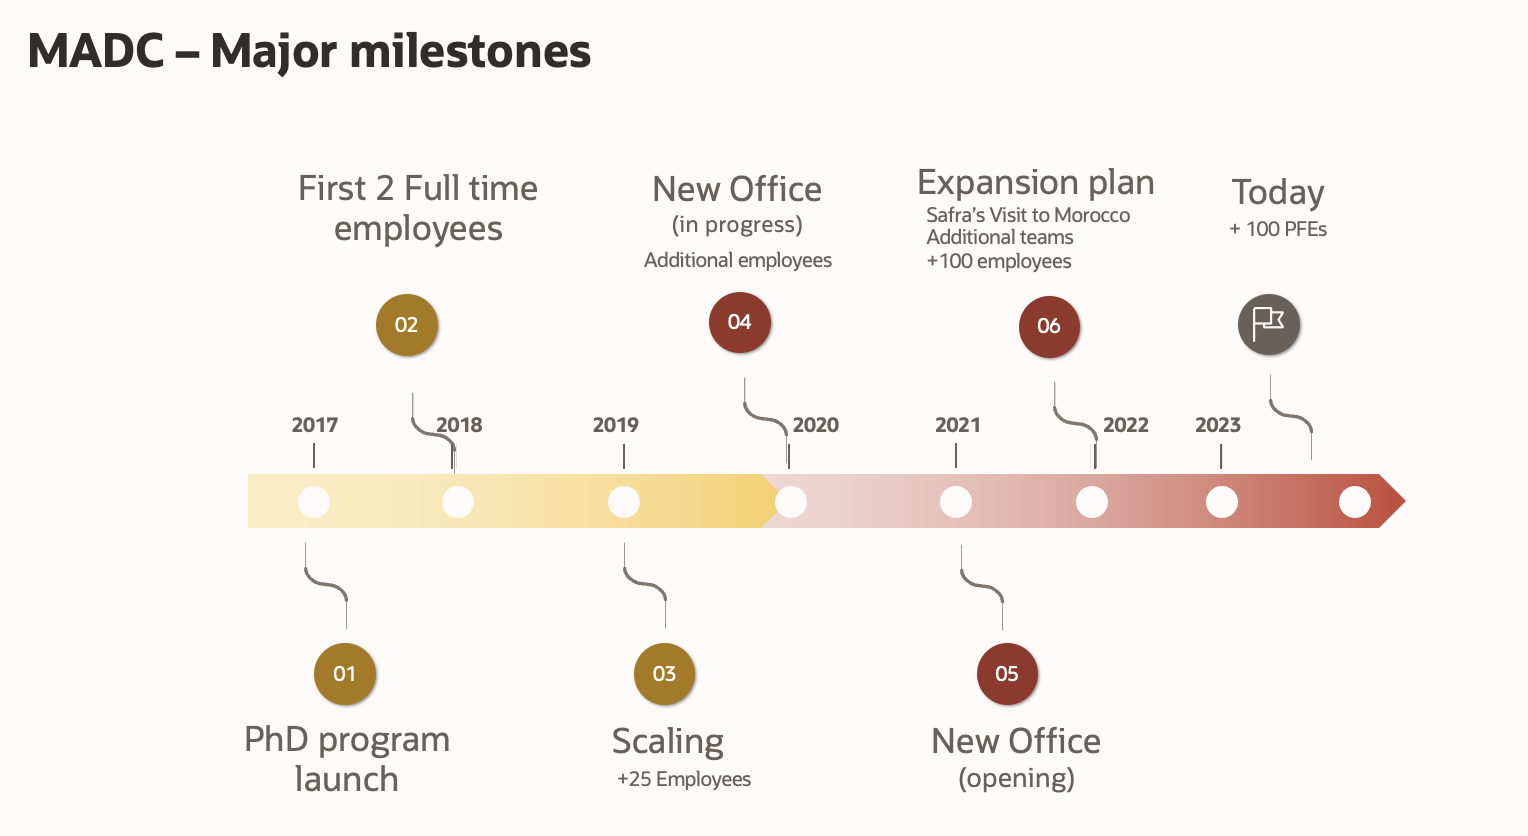
\includegraphics[width=\textwidth]{Images/MADC Major milestones.png}
    \captionof{figure}{MADC Major Milestones}
    \label{fig:madc}
\end{center}
\noindent
\mynewline
The global program includes expanding internship and graduate recruitment initiatives, as well as establishing joint research projects with regional universities.
Oracle MADC has achieved success by delivering several high-quality products and solutions, such as Oracle Cloud Infrastructure (OCI) and Autonomous Data Warehouse (ADW).


% Organizational Structure
\subsection{Organizational Structure}
Oracle Corporation has a hierarchical organizational structure with three main business divisions: Hardware, Services, Cloud and License. Each segment is divided into smaller business units focused on goods, services, or geographical areas. The Board of Directors oversees the company's performance and strategic direction, while the Executive Leadership Team manages daily operations.\mynewline

Functional divisions, including sales, marketing, finance, human resources, legal, and IT, fall under the Executive Leadership Team. Business units are arranged by region, product, and service, with a senior VP or general manager overseeing each unit's operations. The employees are subordinated to both a functional manager and a business unit manager in the matrix-based organizational structure of the business units.\mynewline
\begin{center}
    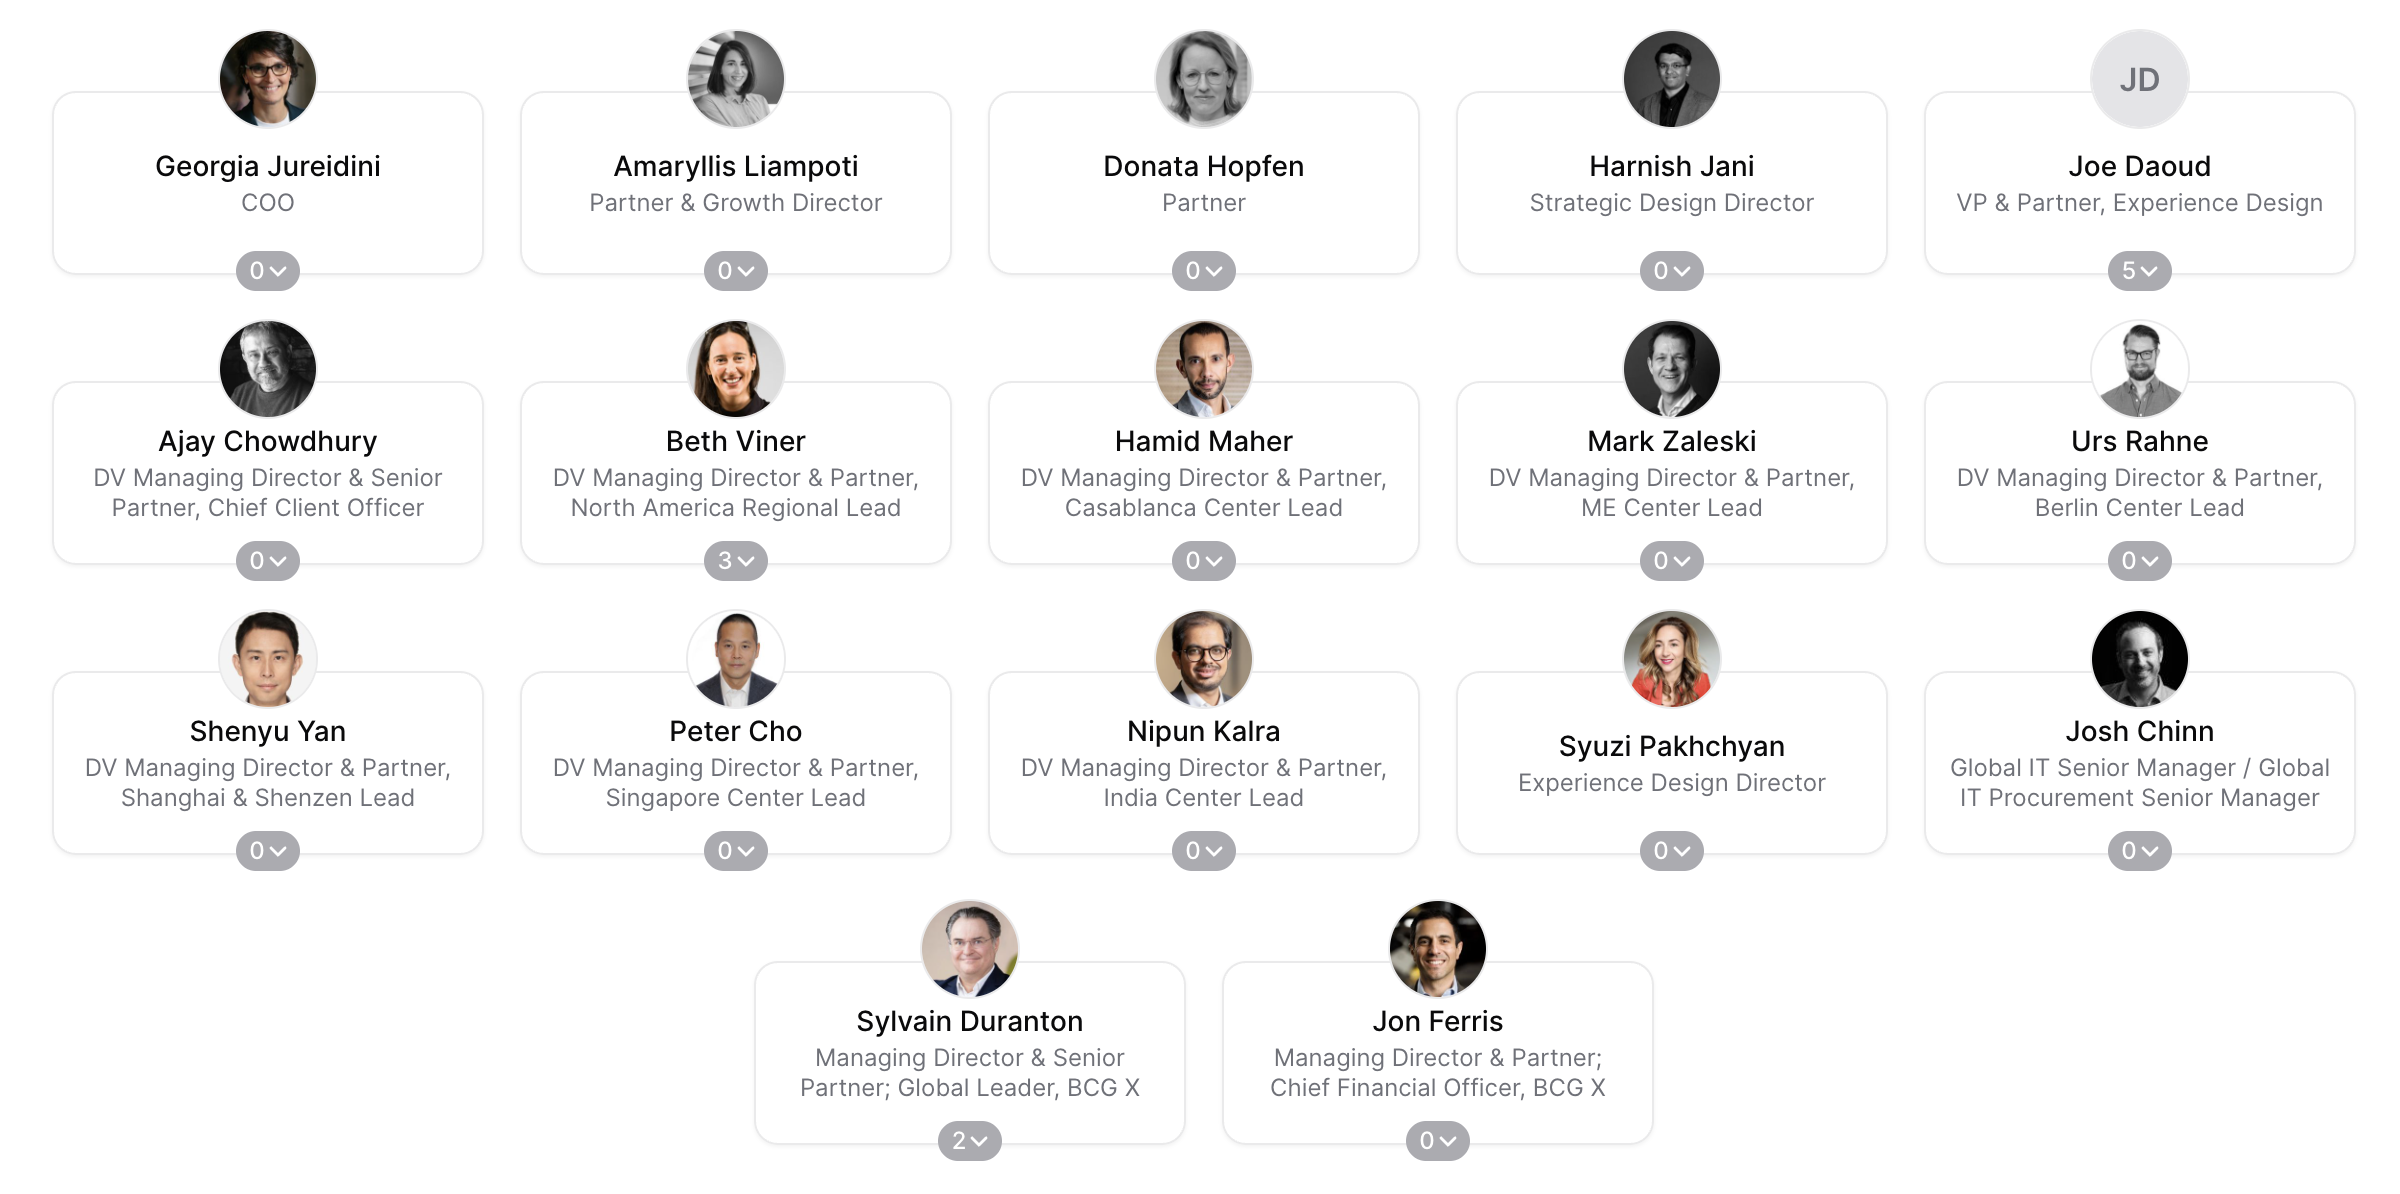
\includegraphics[width=\linewidth]{Images/Executive Leadership Board.png}
    \captionof{figure}{Executive Leadership Board}
    \label{fig:executive}
\end{center}
\noindent
\mynewline
In general, Oracle's organizational structure is built to encourage teamwork, creativity, and client attention. While the matrix form enables people to work across many functions and business divisions to achieve shared goals, the hierarchical structure promotes effective decision-making and communication.

% Organizational Culture
\subsection{Organizational Culture}
Oracle has a strong corporate culture that prioritizes innovation, client focus, and excellence. The company's history of innovation, emphasis on customer satisfaction, and dedication to fostering a friendly and collaborative work environment all have a bearing on the company's culture.\mynewline
Oracle's culture places a strong emphasis on the following:
\begin{itemize}
    \item \textbf{Innovation }\\
          Which is one of its defining characteristics. The business has a lengthy history of creating cutting-edge goods and technology that have revolutionized the tech sector. This culture of innovation is promoted by a dedication to research and development as well as by giving staff members the tools and encouragement they require to test out fresh concepts and create new products.
    \item \textbf{Customer Satisfaction }\\
          Oracle's customer-centric approach to business reflects its commitment to providing goods and services that satisfy the needs of its clients. Employees are encouraged to collaborate closely with clients to comprehend their demands and create solutions that meet their problems.
    \item \textbf{Quality }\\
          Oracle is dedicated to providing quality operations, products, and services, reflected in its solid reputation for quality, dependability, and performance. The company expects every person to strive for excellence, providing them with the tools, resources, and encouragement to succeed.
    \item \textbf{Collaboration and Teamwork }\\
          Effective collaboration is essential for achieving Oracle's goals and delivering value to customers. The company encourages employees to work together across different departments and functions, providing them with tools and resources to facilitate collaboration and communication.
\end{itemize}

Overall, Oracle's organizational culture is characterized by a commitment to innovation, customer focus, excellence, collaboration, and teamwork. These values are reflected in the company's products, services, and operations, and are embraced by its employees at all levels of the organization.


% Project Framework
\section{Project Framework}


% Oracle Linux and Virtualization
\subsection{Oracle Linux and Virtualization}
Oracle Linux is a secure and high-performance operating environment used extensively by thousands of customers worldwide, both in the cloud and on-premises. It powers Oracle Cloud and Oracle Engineered Systems. As an operating system, Oracle Linux provides a solid foundation for virtualization technologies, including Oracle VM and other hypervisors like KVM and Xen. These technologies enable the creation and management of virtual machines (VMs) on Oracle Linux.\mynewline

Oracle Cloud is Oracle's cloud computing platform offering a wide range of services, including infrastructure as a service (IaaS), platform as a service (PaaS), and software as a service (SaaS). Within Oracle Cloud, customers can utilize virtualization capabilities to deploy and manage VMs in a cloud-based environment.\mynewline

The Oracle Linux Virtualization, System, and Hardware Testing team is responsible for ensuring that all virtualization aspects are tested and function as intended before new Oracle Linux releases are submitted or delivered to Oracle Cloud Infrastructure. QA team works closely with the Development team for validating new features, tools etc,  ensuring no regressions occur with previous systems and no bugs, issues, or performance problems arise in future releases. This process includes covering all scenarios and related test cases, and then developing a test plan that encompasses all aspects of the presented and new features.


% Project Context
\subsection{Project Context}
Oracle Linux, as a robust operating system, underpins various virtualization technologies, including Oracle VM, KVM, and Xen. These technologies facilitate the creation and management of virtual machines (VMs) on Oracle Linux. Oracle Cloud, Oracle’s comprehensive cloud computing platform, offers services such as infrastructure as a service (IaaS), platform as a service (PaaS), and software as a service (SaaS). Within this cloud environment, Oracle Linux virtualization serves as a critical bridge, enabling the creation, configuration, and management of VMs. This integration allows businesses to leverage Oracle Linux's stability and flexibility to enhance their cloud computing capabilities.


% Problematic
\subsection{Problematic}
The primary challenge in this project lies in ensuring the compatibility of various virtualization modules (such as QEMU and Libvirt) with different software components. Virtualization modules are intricate systems that interact with multiple hardware and software layers, and updates or new releases can introduce bugs or compatibility issues. For instance, a new version of QEMU might inadvertently introduce defects or regressions, potentially impacting its stability, reliability, and compatibility with existing VM configurations. Ensuring that these components work harmoniously across different versions is crucial to maintaining the functionality and performance of the virtualization environment.

% Objectives
\subsection{Objectives}
To ensure the compatibility and stability of virtualization modules with various software components, this project focuses on validating the correct functioning of QEMU, Libvirt, and other related modules across different releases. These virtualization modules, integral to the Oracle ecosystem, require rigorous testing to maintain their reliability and performance.\mynewline

The objectives are several-fold:
\begin{itemize}
    \item Validate the functionality of QEMU, Libvirt, and other virtualization modules with both new and previous releases of software components such as UEK, Libiscsi, and OVMF;
    \item Implement regression testing to systematically identify and address potential defects or regressions introduced in new software versions;
    \item Ensure the stability, reliability, and compatibility of these virtualization modules across different versions and configurations;
    \item Uphold the core functionalities of the virtualization environment, including virtual machine creation, management, resource allocation, and networking;
    \item Mitigate risks associated with software updates by detecting and resolving issues early in the development cycle.
\end{itemize}

By achieving these goals, we aim to provide a dependable virtualization solution within the Oracle ecosystem, ensuring seamless integration and robust performance for businesses leveraging Oracle Linux virtualization and Oracle Cloud.

% Project Management
\section{Project Management}

% Progress Monitoring
\subsection{Progress Monitoring}
During my internship, we did not strictly adhere to an agile methodology. Instead, we implemented a weekly meeting schedule supplemented by urgent meetings for critical issues, such as troubleshooting problems or addressing pressing concerns. This approach ensured a consistent overview of project developments while allowing for the timely resolution of emergent needs. Additionally, I met one-on-one with my mentor weekly. These meetings allowed me to present the progress made, receive feedback, and discuss any open questions or issues. The feedback provided valuable insights from different perspectives and played a crucial role in refining the project’s functional requirements. Our sync-up meetings typically included status updates, demonstrations of functionality (if applicable), discussion of open questions or issues, and outlining next steps in the project.

% Collaboration Tools
\subsection{Collaboration Tools}
Using collaboration tools within a team offers several benefits. They play an important role in enhancing teamwork and communication within a team, enabling seamless communication through instant messaging and video conferencing. They also facilitate efficient collaboration on shared documents and projects, providing centralized repositories for knowledge sharing and documentation. Here is a list of collaboration tools used during my internship (\textit{Figure~\ref{fig:tools}}):
\begin{center}
    \centering
    
\includegraphics[width=\textwidth]{Images/tools.png}
    \captionof{figure}{Communication Tools}
    Logos from Outlook\cite{Outlook}, Slack\cite{slack}, and Zoom\cite{zoom}.
    \label{fig:tools}
\end{center}
\begin{itemize}
    \item \textbf{\textit{Slack}}: A well-liked platform that offers file transfers, instant messaging, and robust message searching. It integrates with numerous other tools, including Zoom and Outlook, offering interesting features to facilitate communication;
    \item \textbf{\textit{Zoom}}: A cloud-based video conferencing tool that simplifies the  hosting of virtual one-on-one or team meetings. This remote communication tool connects remote team members with one another, providing strong audio, video, and collaboration features;
    \item \textbf{\textit{Outlook}}: Serving as an email management platform, Outlook enables users to send and receive emails, manage calendars, store contact information, and track tasks effectively;
    \item \textbf{\textit{Confluence}}:
          \begin{center}
              \centering
              
\includegraphics[width=0.2\textwidth]{Images/confluence_logo.png}
              \captionof{figure}{Confluence Logo} \cite{Confluence}
              \label{fig:confluence}
          \end{center}
          A collaborative wiki-style platform developed by Atlassian, serving as a central knowledge base and documentation tool. It allows us to document projects comprehensively, ensuring ease of understanding.
\end{itemize}
\subsection{Internship Planning}
My internship was conducted into two phases: the onboarding phase and the project phase.
\subsubsection[Onboarding Phase]{Onboarding Phase}
The first phase was dedicated to onboarding, ensuring a smooth integration into the company and providing the necessary training before starting the project. This phase included several key activities:

\begin{itemize}
    \item \textbf{Account and Software Setup }\\
          The initial step involved setting up various accounts and software essential for daily operations, to ensure we had access to the necessary tools and platforms. This step included also familiarization with the company’s processes and workflows, including understanding the organizational structure and communication tools.
    \item \textbf{Generic Training }\\
          The training provided an excellent opportunity to expand our skills and knowledge in various areas of software development.
          The generic training provided access to Oracle’s learning resources and covered essential tools and platforms, including:
          \begin{itemize}
              \item Communication tools (Slack);
              \item Linux;
              \item Oracle Cloud Infrastructure (OCI);
              \item Developer tools (Git, Bitbucket, Jira);
              \item DevOps;
              \item Scripting;
              \item APEX.
          \end{itemize}
    \item \textbf{Specific Training }\\
          For my specific training, I focused on Oracle Linux and virtualization technologies, as these are essential for our team’s system testing and validation efforts. This training involved gaining more experience in working with Oracle Linux and mastering virtualization tools like QEMU and Libvirt.
\end{itemize}
\subsubsection[Project Phase]{Project Phase}
After the onboarding phase, the focus shifted to the project phase. The following Project Gantt Diagram (\textit{Figure~\ref{fig:gantt}}) illustrates the timeline and sequence of the project phases.

\begin{center}
    \centering
    
\includegraphics[width=\textwidth]{Images/Gantt Diagram.png}
    \captionof{figure}{Gantt Diagram}
    \label{fig:gantt}
\end{center}

\section{Conclusion}
This chapter provided the context of this project. We presented the host organization and discussed the general framework of the project, focusing on its context, problematic, and objectives. We also described  the methodology employed during the internship and the project's planning.